%
% Toronto-RPi-Meetup-2016-01-14.tex
% 
% Copyright (c), 2016 Syed Faisal Akber
%
% All references will be noted in a file called references.txt
%
\documentclass[slidestop,usepdftitle=false,14pt,table]{beamer}
\usepackage[accumulated]{beamerseminar}
\usepackage{beamertexpower}
\usepackage{hyperref}
\usepackage{graphicx}
\usepackage{color}
\usepackage{colortbl}
\usepackage{transparent}

\usepackage[bars]{beamerthemetree}

\usetheme{Madrid}

% Configure Beamer to use the VMware colours
\setbeamercolor{structure}{fg=gray}
\setbeamercolor{example text}{fg=green}
\setbeamercolor{normal text}{fg=white,bg=black}

% Footline chages and remove navigation symbols
\setbeamertemplate{footline}[page number]{}
\beamertemplatenavigationsymbolsempty

% Define title, author and other important information
\title[Raspberry Pi GPIO]
      {Using the GPIO interface on the Raspberry Pi}
%\subtitle{}
\author[S. F. Akber]{Syed Faisal Akber}

% PDF metadata setup
\hypersetup{pdftitle=
  {Using the GPIO interface on the Raspberry Pi},
  pdfauthor={Syed Faisal Akber}}
% Since we're using the background image for the template we don't need to 
% paste the logo everywhere.
\logo{\includegraphics[height=0.8cm]{img/rpi-logo.png}}

% Date of the presentation
\date{2016-01-14}

\begin{document}
% Title page
% Set the background to the title page image
{
%  \setbeamertemplate{background}{\includegraphics[width=\paperwidth,height=\paperheight,keepaspectratio]{template-title0.jpg}}
  \begin{frame}
    \maketitle
  \end{frame}
}

% Insert table of contents (a.k.a. Agenda based upon sections and subsections)
{
%  \setbeamertemplate{background}{\includegraphics[width=\paperwidth,height=\paperheight,keepaspectratio]{template-sectiontitle1.jpg}}
\begin{frame}
  %  \newslide
  \tableofcontents
\end{frame}
}
%% Example flow of a slide/frame
%% \section{A list environment}
%% \frame{
%% \begin{slide}
%% \centerslidesfalse
%% \frametitle{A list environment}

%% \pause
%% \stepwise
%% {%
%%   \begin{description}
%%   \item[foo.] \step{bar.}%%   \step{\item[baz.]} \step{qux.}
%%   \end{description}
%%   }

%% \end{slide}
%%}

% Set the default background for each slide.
%\setbeamertemplate{background}{\includegraphics[width=\paperwidth,height=\paperheight,keepaspectratio]{template-normal.jpg}}

% Start content here
\section{Introduction}
\begin{frame}
\frametitle{Introduction}
\begin{itemize}
\item Raspberry Pi has many interfaces
\item Some we are already familiar with
\item Today we'll look at P1 (GPIO Interface)
\item Its basic usage and pointers to more detail
\end{itemize}
\end{frame}

\section{P1 - GPIO Header}
\begin{frame}[allowframebreaks]
\frametitle{GPIO Pinouts}
\begin{itemize}
\item Each pin has a purpose
\item Power and Ground
\item I/O Pins
\item PWM
\item $I^2C$
\item SPI
\item No analog inputs
\item No analog outputs*
\end{itemize}
\begin{center}
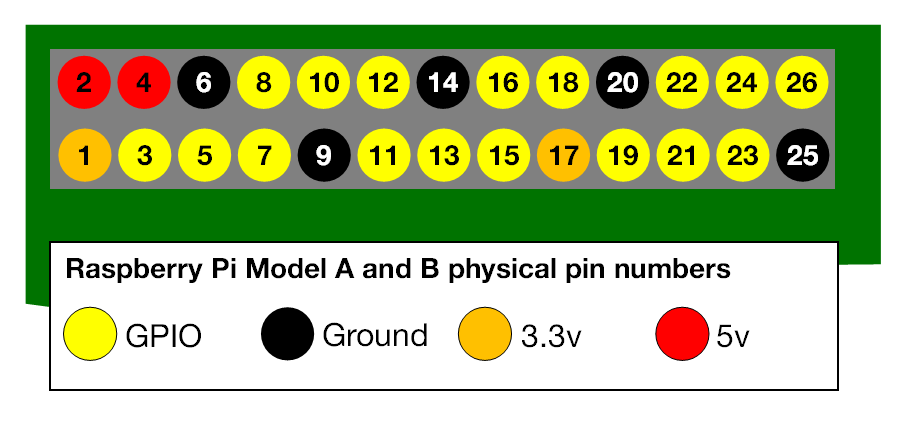
\includegraphics[width=10cm,keepaspectratio]{img/a-and-b-physical-pin-numbers.png}\\
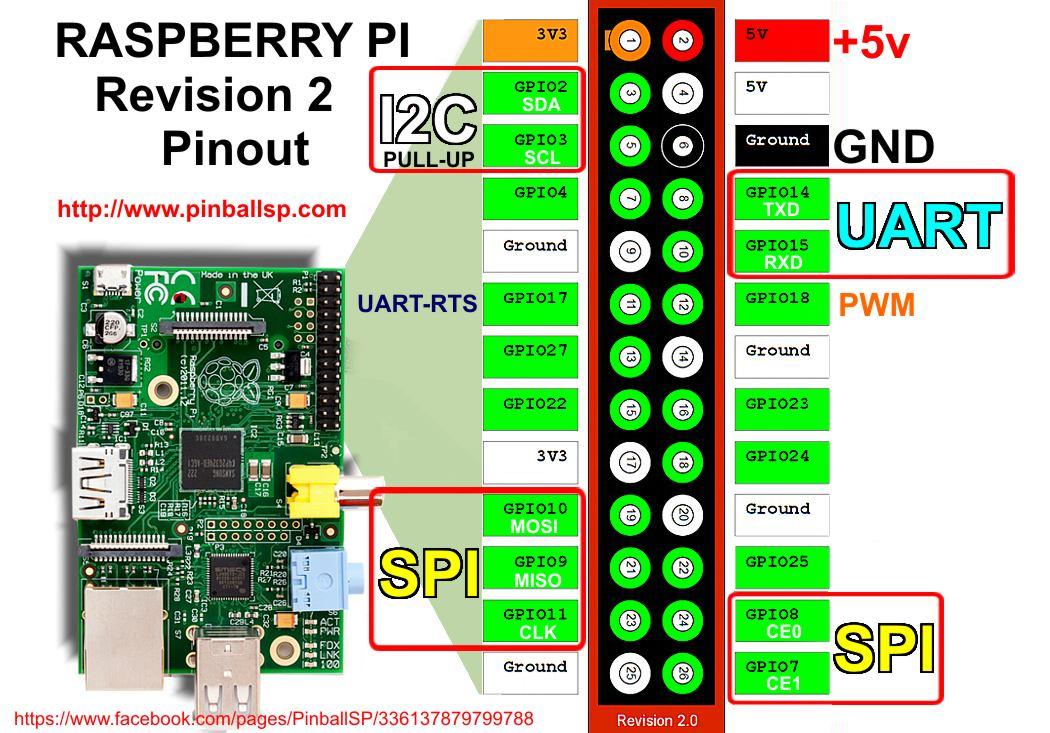
\includegraphics[width=10cm,keepaspectratio]{img/raspberry-pi-rev2-gpio-pinout.jpg}\\
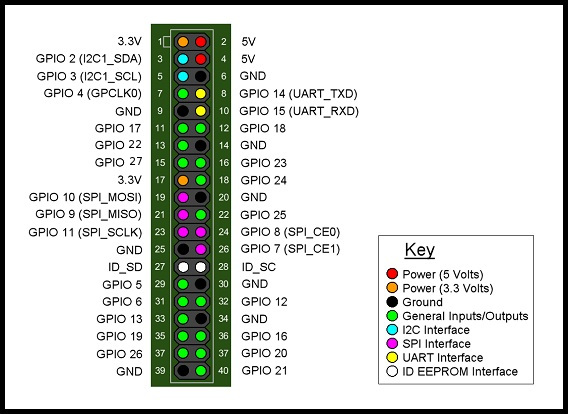
\includegraphics[width=10cm,keepaspectratio]{img/gpio_pinbelegung.jpg}
\end{center}
\end{frame}

\section{Simple I/O}
\begin{frame}[containsverbatim,allowframebreaks]
  \frametitle{Simple Output}
  \begin{itemize}
  \item Simple outputs
    \begin{itemize}
    \item 3.3V if set to 1
    \item 0.0V if set to 0
    \end{itemize}
  \item Easiest to program
  \item Can use Scratch, Python or C
  \item Example\\
    {\tt\small
\begin{verbatim}
import RPi.GPIO as GPIO
import time

GPIO.setmode(GPIO.BCM)
GPIO.setwarnings(False)

ledpin = 18
GPIO.setup(ledpin, GPIO.OUT)

GPIO.output(ledpin, 1)
GPIO.cleanup()
\end{verbatim}
    }

  \end{itemize}
\end{frame}

\begin{frame}[containsverbatim,allowframebreaks]
\frametitle{Simple Input}
\begin{itemize}
\item 3.3V = 1
\item 0.0V = 0
\item Use with buttons and other digital devices
\item Built-in pull up/down resistors
\item Example code\\
    {\tt\small
\begin{verbatim}
btnpin = 18
GPIO.setup(btnpin, GPIO.IN, 
           pull_up_down=GPIO.PUD_DOWN)

while True:
    button = GPIO.input(btnpin)
    if button:
        print('Button pressed')
        time.sleep(0.2) # Debounce
GPIO.cleanup()
\end{verbatim}
    }
\item Debounce switches either in hardware or software using loops
\end{itemize}
\end{frame}

\section{Pulse-Width Modulation (PWM)}
\begin{frame}[containsverbatim,allowframebreaks]
\frametitle{Pulse-Width Modulation (PWM)}
\begin{itemize}
\item PWM creates a pulse of varying widths\\
{\begin{center}
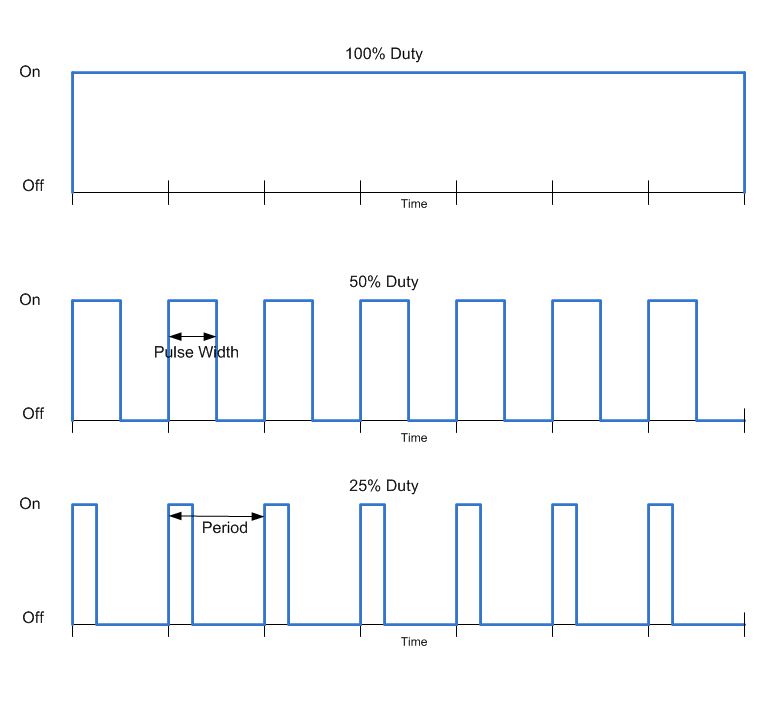
\includegraphics[width=10cm,height=7cm,keepaspectratio]{img/pwm.png}
\end{center}}
\item Dim LED/Lights
\item Control RGB LEDs
\item Contorl motor speed
\item Control servo motors
\item Use as a timing signal
\item Use to broadcast radio signals (PiFM)
\item Example code\\
    {\tt\small
\begin{verbatim}
ledpin = 18
freq = 50 # Hz
GPIO.setup(ledpin, GPIO.OUT)
pwm = GPIO.PWM(ledpin, freq)
pwm.start(25) # duty cycle
time.sleep(5)
pwm.ChangeDutyCycle(75)
time.sleep(5)
GPIO.cleanup()
\end{verbatim}
    }
\end{itemize}
\end{frame}

\section{Serial Communications}
\begin{frame}[allowframebreaks]
  \frametitle{Serial Communications}
  \begin{itemize}
  \item Standard via UART (Pins 8 and 10)
  \item By default, kernel messages and getty are running
  \item Update grub configuration and inittab to disable defaults
  \item To connect RS-232 devices use a MAX3232 to adjust voltages
  \item Other different interfaces exist
    \begin{itemize}
    \item Serial Peripheral Interface (SPI)
    \item Inter-Integrated Circuit ($I^2C$)
    \end{itemize}
  \item Many peripherals use SPI or $I^2C$ such as, LCD Screens and other devices
  \end{itemize}
\end{frame}


\section{Other Topics}
\begin{frame}
  \frametitle{What to do when you're running out of pins!}
  \begin{itemize}
  \item Multiplexing
  \item Specialized hardware drivers (i.e. LED Matrix drivers)
  \item Daisy-chaining 
  \item Add-on boards (Guzunty, Gert, ...)
  \end{itemize}
\end{frame}
  
% Conclusions
%\section{Summary}
%\begin{frame}
%  \frametitle{Summary}
%  \begin{itemize}
%  \item Interfaces
%  \item Pinouts
%  \item Interfacing techniques
%  \item 
%  \end{itemize}
%\end{frame}

% Questions slide
{
%\setbeamertemplate{background}{\includegraphics[width=\paperwidth,height=\paperheight,keepaspectratio]{img/rpi-logo.png}}
\setbeamercolor{structure}{fg=gray}
\begin{frame}
  \frametitle{Questions?}
  \centerslidestrue
\end{frame}
}

% References slide
%\frame{
%  \frametitle{References}
%  \bibliographystyle{abbrvnat}
%  \begin{thebibliography}{}
%    \bibitem[]{RPi}
%      \emph{Raspberry Pi}
%      \url{http://www.raspberrypi.org/}
%    \bibitem[]{RPi-GPIO-pinouts}
%      \emph{GPIO: Raspberry Pi Models A and B}
%      \url{https://www.raspberrypi.org/documentation/usage/gpio/}
%  \end{thebibliography}
%}

\end{document}
